\documentclass{article}

\usepackage{booktabs}
\usepackage{tabularx}
\usepackage{hyperref}
\usepackage{graphicx}

\hypersetup{
    colorlinks=true,       % false: boxed links; true: colored links
    linkcolor=red,          % color of internal links (change box color with linkbordercolor)
    citecolor=green,        % color of links to bibliography
    filecolor=magenta,      % color of file links
    urlcolor=cyan           % color of external links
}

\title{Hazard Analysis\\\progname}

\author{\authname}

\date{}

%% Comments

\usepackage{color}

\newif\ifcomments\commentstrue %displays comments
%\newif\ifcomments\commentsfalse %so that comments do not display

\ifcomments
\newcommand{\authornote}[3]{\textcolor{#1}{[#3 ---#2]}}
\newcommand{\todo}[1]{\textcolor{red}{[TODO: #1]}}
\else
\newcommand{\authornote}[3]{}
\newcommand{\todo}[1]{}
\fi

\newcommand{\wss}[1]{\authornote{magenta}{SS}{#1}} 
\newcommand{\plt}[1]{\authornote{cyan}{TPLT}{#1}} %For explanation of the template
\newcommand{\an}[1]{\authornote{cyan}{Author}{#1}}

%% Common Parts

\newcommand{\progname}{ProgName} % PUT YOUR PROGRAM NAME HERE
\newcommand{\authname}{Team \#, Team Name
\\ Student 1 name
\\ Student 2 name
\\ Student 3 name
\\ Student 4 name} % AUTHOR NAMES                  

\usepackage{hyperref}
    \hypersetup{colorlinks=true, linkcolor=blue, citecolor=blue, filecolor=blue,
                urlcolor=blue, unicode=false}
    \urlstyle{same}
                                


\begin{document}

\maketitle
\thispagestyle{empty}

~\newpage

\pagenumbering{roman}

\begin{table}[hp]
\caption{Revision History} \label{TblRevisionHistory}
\begin{tabularx}{\textwidth}{llX}
\toprule
\textbf{Date} & \textbf{Developer(s)} & \textbf{Change}\\
\midrule
2025-10-09 & All & Created Document\\
\bottomrule
\end{tabularx}
\end{table}

~\newpage

\tableofcontents

~\newpage

\pagenumbering{arabic}

\section{Introduction}

The primary goal of this Hazard Analysis is to identify, categorize, and evaluate potential risks and flaws in the game system and its development process. This proactive approach ensures that we address potential issues before they translate into significant problems during development or post-launch. By maintaining a high standard of quality assurance, we aim to deliver a stable, secure, and enjoyable product. A hazard is a flaw in the system that could lead to the user not enjoying our game, inhibited usability, or security/privacy risks.This document will proceed by identifying various hazards across technical, design, and operational domains. It will then analyze the severity and likelihood of each hazard, assigning a resultant risk level. Finally, for all non-trivial risks, concrete mitigation and contingency plans will be proposed to ensure project integrity and the quality of the final product.\\


\section{Scope and Purpose of Hazard Analysis}

This hazard analysis covers the game software on Windows 10+ (Minimum Spec): input handling (keyboard/mouse; optional gamepad), rendering/audio, terrain \& debris, field publication (water/heat/light), organism traversal, and file I/O (saves/settings/logs). It excludes OS/hardware faults, the Steam client, mods, and online services. Potential future features (e.g., microphone input, external weather) are noted but out of scope for R1.\\

Purpose
\begin{itemize}
\item{Identify hazards arising from normal play and operation}
\item{Rate severity and likelihood to prioritize mitigations}
\item{Turn mitigations into verifiable requirements/tests (tie to SRS E.3/E.6 constraints/invariants and S.6 acceptance).}
\item{Maintain traceability from hazards → requirements → tests.}
\end{itemize}

Potential losses if hazards occur
\begin{itemize}
\item{\textbf{Human health/safety:} photosensitive seizures (flashing), hearing damage (sudden loud audio), motion/visual discomfort. → Loss: injury or illness.}
\item{\textbf{Accessibility/usability:} unreadable UI at 1280×720; non-functional keyboard/mouse paths. → Loss: players can’t play/progress.}
\item{\textbf{Data integrity:} corrupted/partial saves/settings/logs. → Loss: progress/time loss; inability to resume.}
\item{\textbf{Privacy (future features):} unintended microphone capture/storage. → Loss: personal data exposure; reputational harm.}
\item{\textbf{Stability/performance:} crashes, hangs, excessive resource use, high latency. → Loss: denial of service; unplayable experience.}
\item{\textbf{Legal/compliance:} mis-licensed assets; writing outside user-writable paths. → Loss: policy violations; takedowns.}
\item{\textbf{Project/academic outcome:} failure to meet Minimum Spec or acceptance criteria. → Loss: missed milestones; grading/demo impact.}
\end{itemize}

Method (summary)
Use a checklist + what-if sweep and a simple severity/likelihood matrix (Low/Med/High). For each high/medium risk, define a concrete mitigation that becomes a testable requirement in S.6 (e.g., “atomic save writes,” “publish $\leq$ 1.0 s,” “readable at 1280×720”). 

\section{System Boundaries and Components}

1. Debris System\\

2. Inventory System\\

3. Player Controller\\

4. Organic Pathway System\\


\section{Critical Assumptions}

This section outlines the foundational assumptions made about the project's development environment, technical stability, and external dependencies. A failure in any of these assumptions must trigger an immediate re-evaluation of the project plan and hazard analysis.\\

A core assumption is the technical feasibility of the core requirements. We assume the specialized systems, the destructible environment and the slime mold traversal system, can be implemented successfully using the chosen engine and tools within the timeframe established by Sprint 0. Discovering fundamental limitations after that initial sprint will necessitate a critical reduction in the project's overall scope.\\

We also assume the stability of the development environment. This means the chosen game engine and all associated third-party components (such as physics libraries) will remain stable, compatible, and maintainable throughout the entire development cycle, from Sprint 0 through Sprint 3. We assume there won't be any major, unscheduled, or breaking changes to the engine or dependencies during this time.\\

The project relies on the availability of human resources. We assume that all core development team members will be available and committed to the project according to the schedule in P.4 of the SRS document. The successful delivery of key sprint items would be compromised if any critical team member experienced a prolonged, unplanned absence.\\

We make assumptions regarding user system specifications. We assume the final game will be run on hardware and operating systems that meet the minimum specifications to be defined in the Design Document (Revision 0). We manage performance hazards based on the expectation that end-users possess at least these minimum required specifications.\\

\section{Failure Mode and Effect Analysis}

\begin{figure}[h!]
	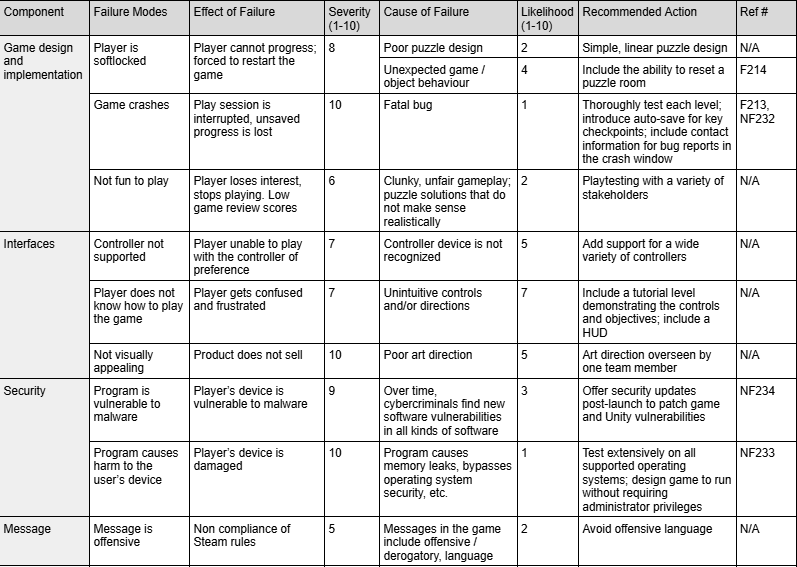
\includegraphics[width=\linewidth]{FMEA.png}
\end{figure}

\section{Safety and Security Requirements}

\begin{itemize}
\item{System must experience crashes no more frequently than once every two hours on average.}
\item{System must be able to run without requiring administrator privileges.}
\item{Autosaves should happen at the start of new levels and at key checkpoints on each level.}
\item{Any Unity security vulnerabilities should be patched in a timely fashion.}
\item{Crash log should be adequately informative and detailed.}
\item{Avoid offensive language.}
\item{Offer security updates post-launch.}
\item{Have an ingame Heads-Up Display.}
\item{Have a tutorial level.}
\item{Support a wide variety of controllers.}
\item{Contact information for bug reporting in the built-in crash window.}
\item{Auto-save feature.}
\end{itemize}

\section{Roadmap}

All requirements in regards to validating correct and expected behavior of the destructible environment and organic pathway system should be implemented and met by the proof of concept stage in addition to the basic UI organization as well as making sure any hardware and/or potential internet vulnerability countermeasures are implemented. \\

Once the core mechanics of the project are solidified, the game levels can be built and tested over top of that and evaluated on usability and adherence to the central theme of the game. Each level should also be built based on the core mechanics of the game\\


\newpage{}

\section*{Appendix --- Reflection}

\textbf{Team:}\\

3. Before beginning this deliverable, we thought of risks such as:\\
-The game not being fun, or not being visually appealling\\
-Controller support\\
The rest came about by imagining ourselves playing our game and thinking about what could go wrong at any step of the gameplay loop. It also came from thinking about our past experiences playing other games that had bugs or other issues. This led to thoughts of softlocks, crashes, lost save data, and so on.\\

\textbf{Felix Hurst}
\begin{enumerate}
\item{After defining what a “hazard” is in the context of our project, it became easy to come up with potential hazards, creating the FMEA table smoothly with a few categories for organization.}
\item{Because our project is a game, it is difficult to define “hazards” for a system that has no chance of physically harming the user. We resolved this by redefining what a “hazard” is in the context of our system. Now they focus on security risks, usability, and user enjoyment. This allows us to have a better perspective of “what could go wrong” in the development of our system.}
\item{See team answer above.}
\item{Two other types of risks in software products include:\\
Data privacy: Will the system collect a user’s personal information? If so, it should be kept safe, protected from being leaked to malicious third parties.\\
Malware vulnerability: Does the system have any extreme weaknesses that could be exploited to enable an attacker to cause harm to the user’s device? Care should be taken to keep a program as secure as possible.}
\end{enumerate}

\textbf{BoWen Liu}
\begin{enumerate}
\item{Our team was able to efficiently identify what would be defined as a “hazard” in our project and set out a plan based on our deliverable schedules as to the concrete implement details.}
\item{In contrast to projects that require internet connection and/or multiple users, our game is fairly closed off as a package with minimum possible network weaknesses, however we were able to identify unique failure points that are unique to our game project such as game breaking bugs and potential third party vulnerabilities with Unity.}
\item{See team answer above.}
\item{Risks may include for our case security vulnerabilities in 3rd party software that we use in our case Unity, Another risk could be game breaking bugs resulting in the player unable to proceed to the next level thereby making the player stuck at a level.}
\end{enumerate}

\textbf{Marcos Hernandez-Rivero}
\begin{enumerate}
\item{Many of the sections were not too hard to write, and I found that after we met up as a group and discussed some things (like defining what we consider to be a hazard), it became a lot easier to write a given section, since this document is fairly straight forward.}
\item{For us, "Hazards" sounded a bit harsh, and given that we are making a game, we did not really see (at first) how a game could have "hazards" apart from a memory leak affecting the computer, especially since we do not intend to make this an online game, so the user's communication with external parties is VERY limited.}
\item{See team answer above.}
\item{One such risk is a memory leak, where a program consumed more and more memory due to not closing off access to the memory, eventually affecting the entire computer's performance if it goes on long enough. Another suck risk would be malware. We plan to release this game on the Steam platform which does verify files for malware and is widely known and trusted, but at the end of the day, we are not the ones hosting the game, and a malicious actor in Steam's system may be able to change our game files and add in malware. These risks are important to consider because they are sometimes invisible, it's almost impossible to tell just from looking at a screen if a memory leak is happening or if a virus is on your computer until it has already acted and caused severe damage, thus we must ensure that we are very careful to not introduce these risks.}
\end{enumerate}

\end{document}